\subsection{ResNet-50 on CIFAR100}\label{cifar-100-results}

\begin{tabularx}{\textwidth}[hb]{*{2}{>{\centering\arraybackslash}X}}
    \centering
    \captionsetup{labelformat=andfigure,width=1\linewidth,aboveskip=7pt,belowskip=0pt}
    \captionlistentry[figure]{entry for figure}
    \label{fig:cifar100-main-results}
    
    \captionof{table}{\textbf{Benchmarking sparse ResNet-50s on CIFAR-100,} tabulated by performance and cost \textbf{(below)}, and plotted across densities \textbf{(right)}. In each group below, \textit{RigL} outperforms or matches existing sparse-to-sparse and dense-to-sparse methods. Notably, \textit{RigL}\textsubscript{$3\times$} at 90\% sparsity and \textit{RigL}\textsubscript{$2\times$} at 80\% sparsity surpass iterative pruning with similar FLOP consumption. \textit{RigL}\textsubscript{$2\times$} (ERK) further improves performance but requires a larger training budget. }
    \resizebox{1.15\linewidth}{!}{%
\begin{tabular}{ c cc cc }
\toprule
\multirow{3}{*}{\textbf{Method}}& 
\multicolumn{2}{c}{$\mathbf{1 - s=0.1}$} & \multicolumn{2}{c}{$\mathbf{1 - s=0.2}$} \\
\cmidrule(lr){2-3} \cmidrule(lr){4-5}
{} & 
\makecell{Accuracy $\uparrow$ \\ (Test)}  & \makecell{FLOPs $\downarrow$  \\ (Train, Test)} &
\makecell{Accuracy $\uparrow$ \\ (Test)}  & \makecell{FLOPs $\downarrow$  \\ (Train, Test)} \\
\midrule
Static & 
{69.7 $\pm$ 0.42} & {0.10x, 0.10x} & 
{72.3 $\pm$ 0.30} & {0.20x,0.20x} \\

Small Dense & 
{70.8 $\pm$ 0.22} & {0.11x, 0.11x} & 
{72.6$\pm$ 0.93} & {0.20x, 0.20x} \\

SET &
{71.4 $\pm$ 0.35} & {0.10x, 0.10x} & 
{73.4 $\pm$ 0.45} & {0.20x, 0.20x} \\

\textbf{RigL} &
\textbf{71.8 $\pm$ 0.33} & {0.10x, 0.10x} &
\textbf{73.5 $\pm$ 0.04} & {0.20x, 0.20x} \\
\midrule

Static (ERK) & 
{71.5 $\pm$ 0.18} & {0.22x, 0.22x} & 
{73.2 $\pm$ 0.39} & {0.38x, 0.38x} \\

SET (ERK)&
{72.3 $\pm$ 0.39} & {0.22x, 0.22x} &
\textbf{73.5 $\pm$ 0.25} & {0.38x, 0.38x} \\

\textbf{RigL (ERK)} &
\textbf{72.6 $\pm$ 0.37} & {0.23x, 0.22x} &
{73.4 $\pm$ 0.15} & {0.38x, 0.38x} \\
\midrule

SNFS & 
{72.3 $\pm$ 0.20} & {0.58x, 0.37x} & 
{73.9 $\pm$ 0.20} & {0.70x, 0.55x} \\ 

SNFS (ERK)& 
{73.0 $\pm$ 0.33} & {0.59x, 0.38x} & 
{73.9 $\pm$ 0.27} & {0.69x, 0.54x} \\

{Pruning} & 
{73.1 $\pm$ 0.32} & {0.36x,0.11x} & 
{73.8 $\pm$ 0.23} & {0.45x,0.25x} \\ 

{RigL\textsubscript{$2 \times$}} &
{73.1 $\pm$ 0.71} & {0.20x, 0.10x} &
{74.0 $\pm$ 0.24} & {0.41x, 0.20x} \\

{Lottery} &
{73.6 $\pm$ 0.32} & {0.62x,0.11x} & 
{74.2 $\pm$ 0.41} & {0.81x,0.25x} \\

\textbf{RigL\textsubscript{$3 \times$}} &
\textbf{73.7 $\pm$ 0.16} & {0.30x, 0.10x} &
{74.2 $\pm$ 0.23} & {0.61x, 0.20x} \\

\textbf{RigL\textsubscript{$2 \times$} (ERK)} &
{73.6 $\pm$ 0.05} & {0.46x, 0.22x} &
\textbf{74.4 $\pm$ 0.10} & {0.76x, 0.38x} \\

\midrule

\textbf{Dense Baseline} &
\textbf{74.7 $\pm$ 0.38} & {7.77e9, 2.59e9} &
\textbf{-} & {-} \\
\bottomrule

\end{tabular}%
}

    \label{tab:cifar100-main-results}  
&
    \centering
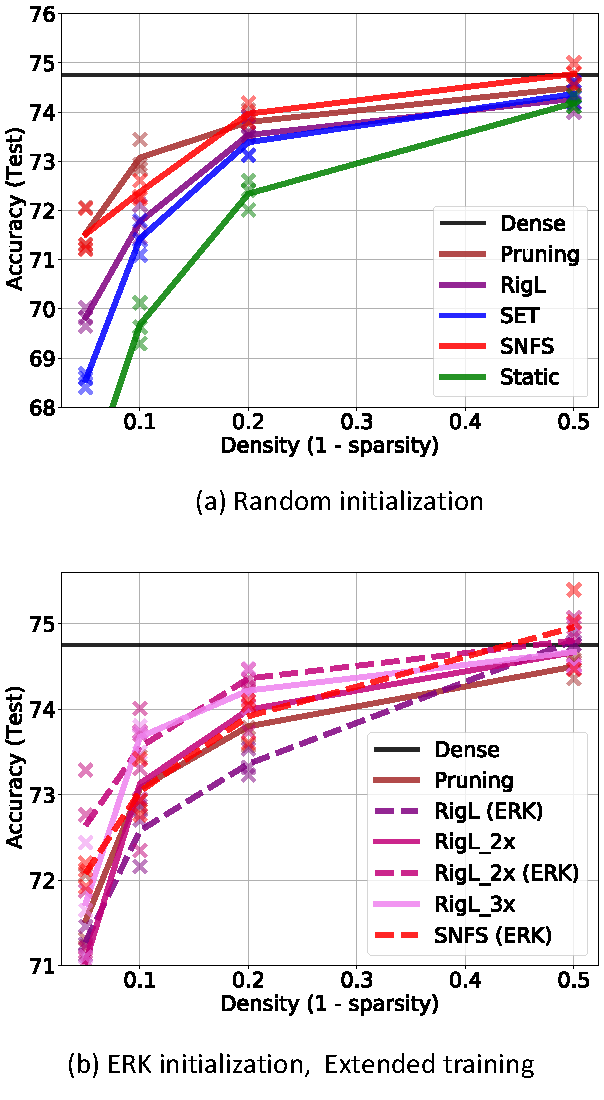
\includegraphics[width=0.66\linewidth,valign=t]{../openreview/figs/cifar100_main.pdf}
\end{tabularx}

We see similar trends when training sparse variants of ResNet-50 on the CIFAR-100 dataset (Table \ref{tab:cifar100-main-results}, metrics reported as in Section \ref{cifar-10-results}). We also include a comparison against sparse networks trained with the Lottery Ticket Hypothesis (\citet{frankle2018lottery}) in Table \ref{tab:cifar100-main-results}---we obtain tickets with a commensurate performance for sparsities lower than 80\%. Finally, the choice of initialization scheme affects the performance and FLOP consumption by a greater extent than the method used itself, with the exception of SNFS (groups 1 and 2 in Table \ref{tab:cifar100-main-results}). 

% Such networks are trained twice: once to prune the dense model, and then after re-initializing with the obtained mask. Finally, concurring with \citet{rigl}, multiple sparse methods generalize better than the dense baseline with just half the parameters, indicating the regularization aspect of sparse networks (Figure \ref{fig:cifar100-main-results}, bottom).  

% ERK initialization improves performance across all sparse methods, especially at higher sparsities. 

